% Description of the paper meetings and their explanation

\section{Meetings}
Retaining the exact same number of players, each generation, requires rounding up the emerging number of players each strategy has at the end of each generation and then redistributing the decimal parts. Ultimately, the decimal parts in our 3-strategy meetings add up to either one or two, and the distribution method we found to be the most fair was:
\begin{itemize}
    \item If the remainder sum is 1, we round up each strategy to the previous integer and distribute the decimal part to the strategy that is the closest to its next integer.
    \item If the remainder sum is 2, we round up each strategy to the previous integer and distribute the decimal part to the two strategies that are the closest to their next integer. 1 to each.
    \item If the remainder sum is 0, there are no decimal parts.
\end{itemize}
We also devised a similar method which, this time, distributes the decimal parts to the top two strategies in terms of total population. We used both methodologies to conduct our experiments. However, when comparing our results with the 1999's paper "Studies on Dynamics in the Classical Iterated Prisoner's Dilemma with Few Strategies" the graphs we produced were mostly coherent but ultimately different. These differences can be largely attributed to the mutable nature of the simulations hidden in programming layers of abstraction and the non-disclosed method of rounding used by the authors of the paper. They only stated that: "All divisions being rounded to the nearest lower integer.", which is not accurate based on their results which seem to be retaining their initial total population. This will be an attempt to replicate the paper's results while attributing our differences and trying to make the same point the original authors were trying to make regardless of the differences. Here is our rounding logic: 
\begin{}
%%%%%%%% DECIMAL REDISTRIBUTION %%%%%%%%%%%%%
if rounding == "pop"
    remainder = zeros(1, length(strategies));

    for i = 1:length(strategies)
        Wn(i) = totalplayers * Gn(i)*Wn(i) / Tn;
        remainder(i) = Wn(i) - floor(Wn(i));
        Wn(i) = floor(Wn(i));
    end

    remaining = totalplayers - sum(Wn);  % How many individuals to redistribute
    [~, sortedIndices] = sort(Wn, 'descend');  % Sort by largest populations

    for k = 1:remaining
        Wn(sortedIndices(k)) = Wn(sortedIndices(k)) + 1;
    end
end
if rounding == "dec"
    remainder = zeros(1, length(strategies));

    for i = 1:length(strategies)
        Wn(i) = totalplayers * Gn(i) * Wn(i) / Tn;
        remainder(i) = Wn(i) - floor(Wn(i));
        Wn(i) = floor(Wn(i));
    end

    remaining = totalplayers - sum(Wn);  % How many individuals to redistribute
    [~, sortedIndices] = sort(remainder, 'descend');  % Sort by largest decimals

    for k = 1:remaining
        Wn(sortedIndices(k)) = Wn(sortedIndices(k)) + 1;
    end
end            
if rounding == "off"
    for i = 1:length(strategies)
        Wn(i) = totalplayers * Gn(i)*Wn(i) / Tn;
    end
end
\end{}
It is important to note that when comparing equal quantities there is no clear ranking between remainders. Thus the program decides where to distribute the decimal parts based on the order of the strategies. This could very well be consequential enough to skew the results in a different direction. Let's see how our results compare relative to the ones in the paper.

\subsection{Defectors may be strong}
This meeting is supposed to show how defecting more often can be beneficial, for the defector, in chaotic environments. When rounding using the "dec" method we observe oscillations that converge to a stable state. 
\begin{figure}[H]
    \centering
    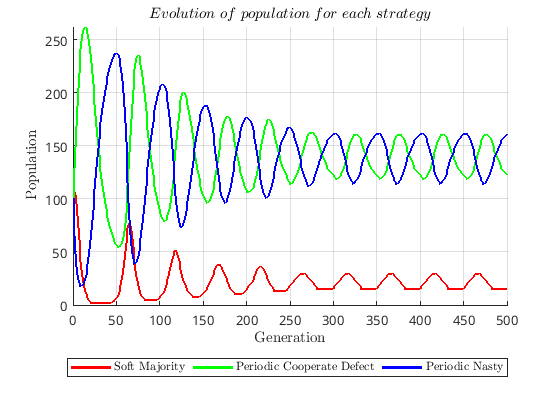
\includegraphics[width=0.8\textwidth]{media/meetings/defectors_may_be_strong_dec.png}
    \caption{Defectors may be strong Dec Plot}
\end{figure}
When rounding using the "pop" method we replicate the results of the paper.
\begin{figure}[H]
    \centering
    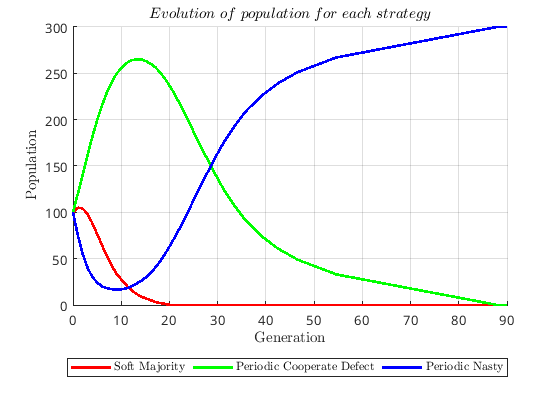
\includegraphics[width=0.8\textwidth]{media/meetings/defectors_may_be_strong_pop.png}
    \caption{Defectors may be strong Pop Plot}
\end{figure}

\subsection{Monotonous convergence}
This meeting simulates clear monotonous convergence. The paper claims this is the most common outcome of the experiments they ran. Here both "pop" and "dec" methods produced identical results recreating the paper's plots. 
\begin{figure}[H]
    \centering
    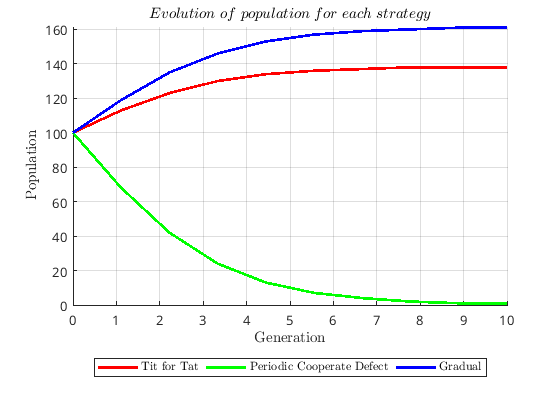
\includegraphics[width=0.8\textwidth]{media/meetings/monotonous_convergence_dec.png}
    \caption{Monotonous convergence Dec Plot}
\end{figure}

\subsection{Attenuated oscillatory movements}
Here we see decreasing oscillations that reach an equilibrium. Both rounding methods are again very close to the paper.
\begin{figure}[H]
    \centering
    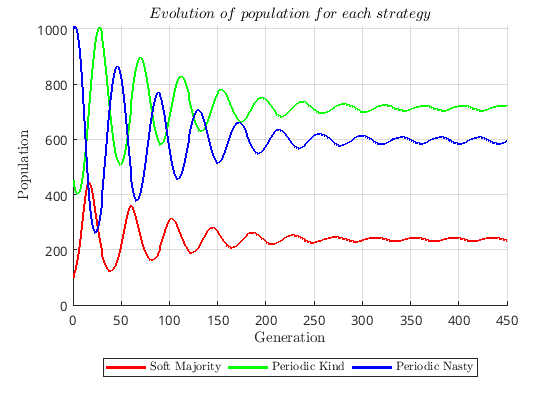
\includegraphics[width=0.8\textwidth]{media/meetings/attenuated_oscillatory_movements_dec.png}
    \caption{Attenuated oscillatory movements Dec Plot}
\end{figure}

\subsection{Periodic movements}
The periodic movements meeting highlights the periodicity and constant amplitude of the oscillations. The "dec" rounding method comes closest to replicating the paper's results.
\begin{figure}[H]
    \centering
    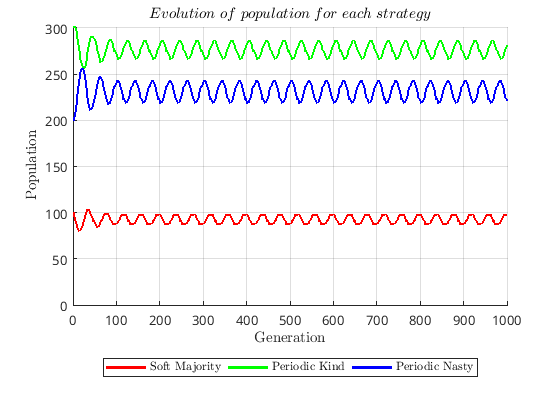
\includegraphics[width=0.8\textwidth]{media/meetings/periodic_movements_dec.png}
    \caption{Periodic movements Dec Plot}
\end{figure}
Using the "pop" method increased the amplitude of the oscillations.
\begin{figure}[H]
    \centering
    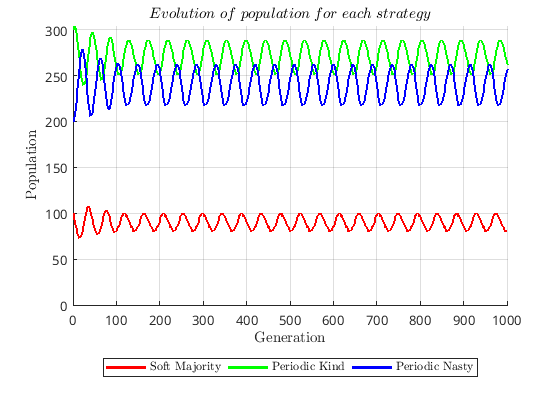
\includegraphics[width=0.8\textwidth]{media/meetings/periodic_movements_pop.png}
    \caption{Periodic movements Pop Plot}
\end{figure}

\subsection{Increasing oscillations}
We were unable to replicate these results. The oscillations seem to converge in all three rounding methods we used. Here is the "dec" method's result.
\begin{figure}[H]
    \centering
    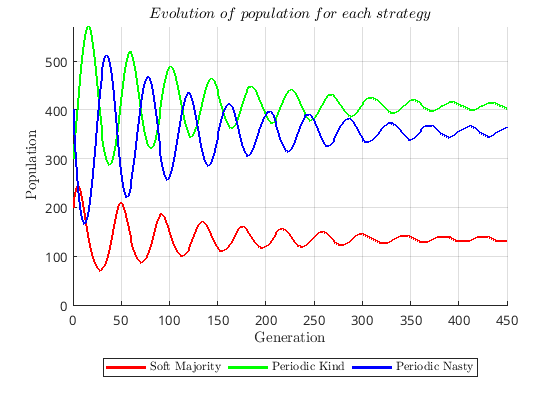
\includegraphics[width=0.8\textwidth]{media/meetings/increasing_oscillations_dec.png}
    \caption{Increasing oscillations Dec Plot}
\end{figure}

\subsection{Disordered oscillations}
When examining the disordered oscillations, the closest we could get was the "off" method. However the phenomenon ended quicker, at around 260 generations and the final state had soft majority and periodic ultra kind strategies go extinct. "dec" and "pop" had very similar behavior to the attenuated oscillatory movements meeting.
\begin{figure}[H]
    \centering
    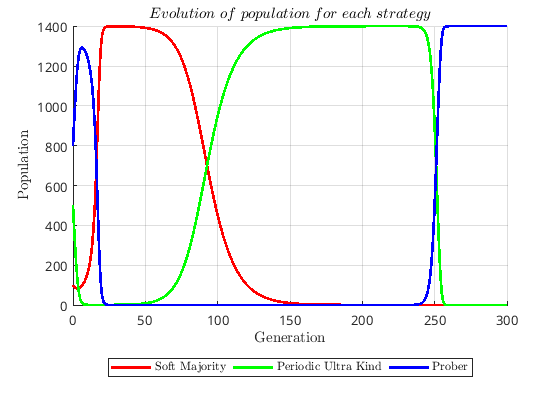
\includegraphics[width=0.8\textwidth]{media/meetings/disordered_oscillations_off.png}
    \caption{Disordered oscillations off Plot}
\end{figure}

\subsection{Population size sensitivity}
Going forward the paper decides to explore the tournament's sensitivity in slight changes of various parameters starting with the initial population size. Other than the fact that the crucial point where the oscillations stop gets shifted at per_ddc population: 235 into 236, instead of 244 into 245, the plots are the same. The rounding method used is "dec".
\begin{figure}[H]
    \centering
    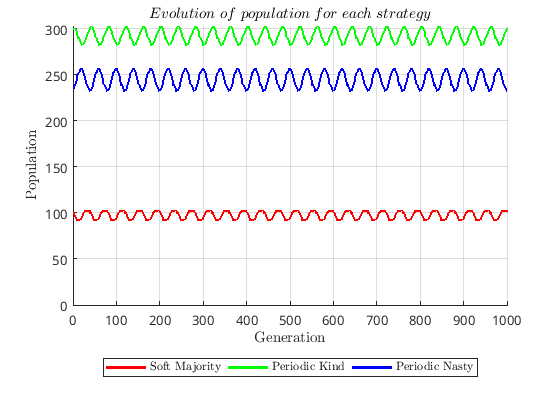
\includegraphics[width=0.8\textwidth]{media/meetings/population_size_sensitivity_before_dec.png}
    \caption{Population size sensitivity before Dec Plot}
\end{figure}
\begin{figure}[H]
    \centering
    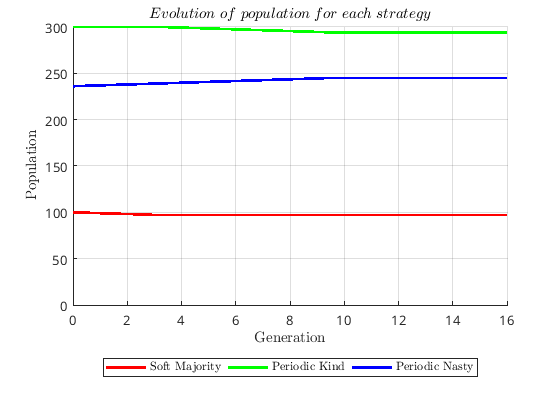
\includegraphics[width=0.8\textwidth]{media/meetings/population_size_sensitivity_after_dec.png}
    \caption{Population size sensitivity after Dec Plot}
\end{figure}

\subsection{Population size sensitivity 2}
The second population sensitivity experiment appears to have the same shift where this time, 159 into 160 becomes 181 into 182. The rounding method used is "pop".
\begin{figure}[H]
    \centering
    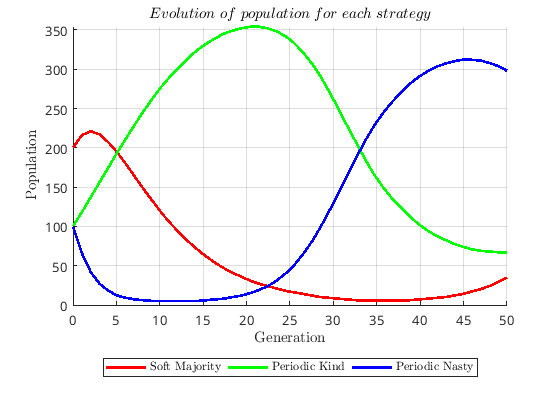
\includegraphics[width=0.8\textwidth]{media/meetings/population_size_sensitivity_2_before_pop.png}
    \caption{Population size sensitivity 2 before Pop Plot}
\end{figure}
\begin{figure}[H]
    \centering
    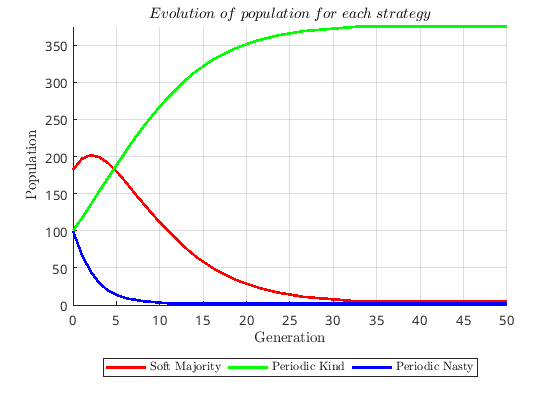
\includegraphics[width=0.8\textwidth]{media/meetings/population_size_sensitivity_2_after_pop.png}
    \caption{Population size sensitivity 2 after Pop Plot}
\end{figure}

\subsection{Game length sensitivity}
This experiment examines the case of changing the game's length or the number of rounds played by the players each generation. In the before state the reach higher peaks in the paper than our example, however we manage to capture the transition from periodic movements to attenuated oscillations. The rounding method used is "dec".
\begin{figure}[H]
    \centering
    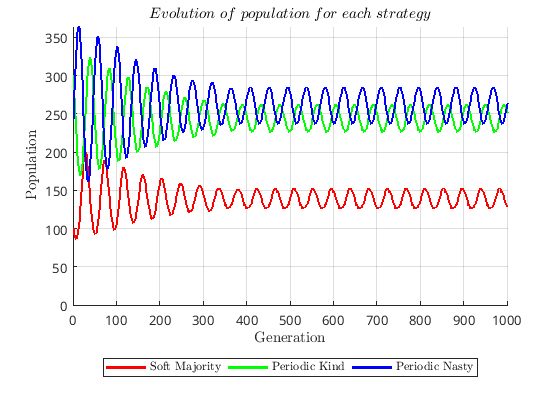
\includegraphics[width=0.8\textwidth]{media/meetings/game_length_sensitivity_before_dec.png}
    \caption{Game length sensitivity before Dec Plot}
\end{figure}
\begin{figure}[H]
    \centering
    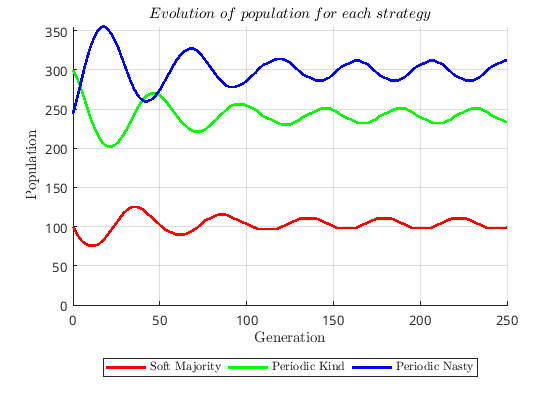
\includegraphics[width=0.8\textwidth]{media/meetings/game_length_sensitivity_after_dec.png}
    \caption{Game length sensitivity after Dec Plot}
\end{figure}

\subsection{Payoff matrix sensitivity}
This meeting highlights the effects a slight change to one of the payoff matrix values can have on the results. In the before state we see increasing oscillations and after changing the defector's exploiting payoff these oscillations become periodic. We perfectly replicate the paper's results using the "dec" method. 
\begin{figure}[H]
    \centering
    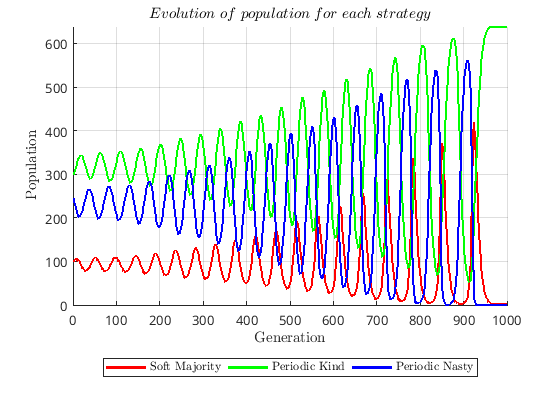
\includegraphics[width=0.8\textwidth]{media/meetings/payoff_matrix_sensitivity_before_dec.png}
    \caption{Payoff matrix sensitivity before Dec Plot}
\end{figure}
\begin{figure}[H]
    \centering
    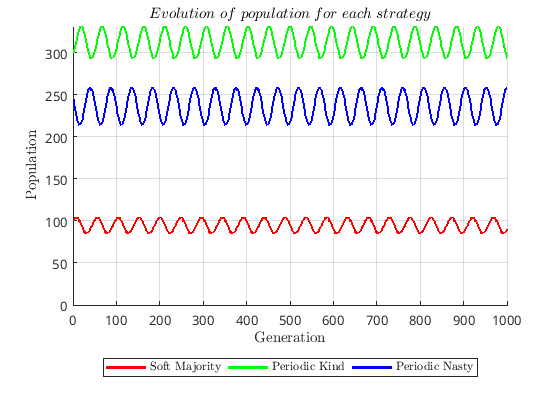
\includegraphics[width=0.8\textwidth]{media/meetings/payoff_matrix_sensitivity_after_dec.png}
    \caption{Payoff matrix sensitivity after Dec Plot}
\end{figure}

\subsection{Rounding method sensitivity}
The final category of minor changes leading to different results is the rounding method. Though out the meetings analysis we have highlighted the importance of the rounding method since to replicate the paper's results we resorted to creating more than one methods, alternating between all of them to better illustrate the effects mentioned in the paper. On the first example we see periodic movements become attenuated oscillations and ultimately steady states. The rounding method used in the before state is "dec" and in the after state it is "off" or no rounding.
\begin{figure}[H]
    \centering
    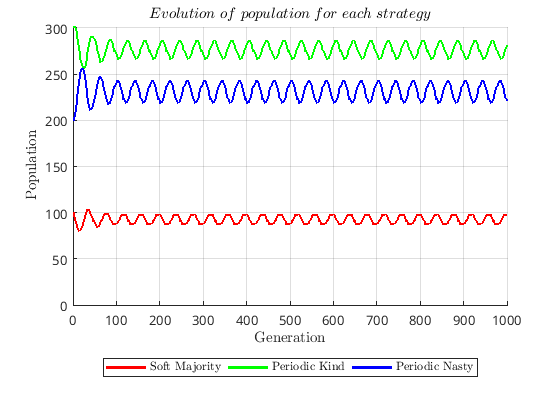
\includegraphics[width=0.8\textwidth]{media/meetings/rounding_method_sensitivity_before_dec.png}
    \caption{Rounding method sensitivity before Plot}
\end{figure}
\begin{figure}[H]
    \centering
    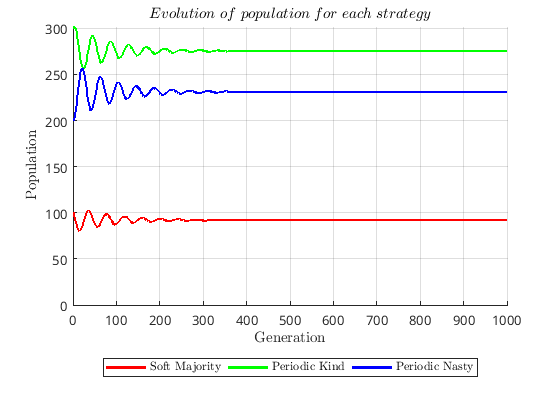
\includegraphics[width=0.8\textwidth]{media/meetings/rounding_method_sensitivity_after_off.png}
    \caption{Rounding method sensitivity after Plot}
\end{figure}
The second example is best displayed using the "pop" method. Here we divide our initial populations with ten making rounding more important since we round an substantially larger section of the individual populations.
\begin{figure}[H]
    \centering
    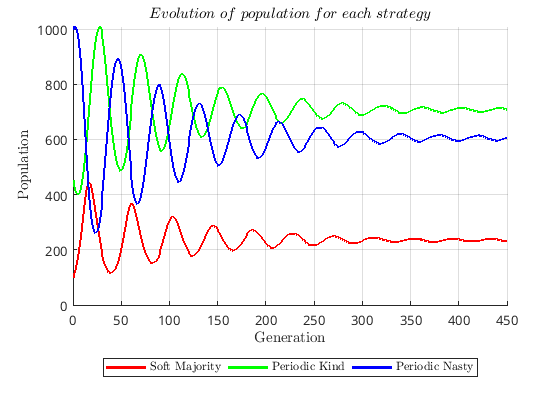
\includegraphics[width=0.8\textwidth]{media/meetings/rounding_method_sensitivity_2_before_pop.png}
    \caption{Rounding method sensitivity 2 before Plot}
\end{figure}
\begin{figure}[H]
    \centering
    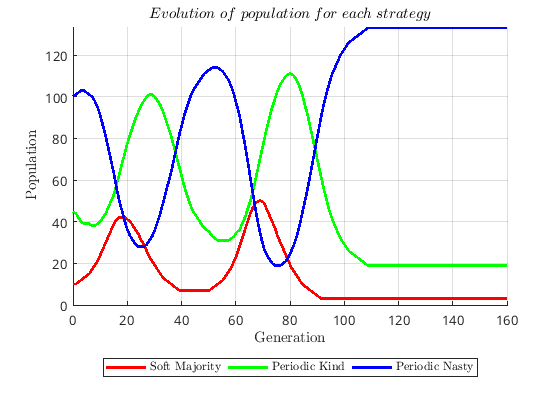
\includegraphics[width=0.8\textwidth]{media/meetings/rounding_method_sensitivity_2_after_pop.png}
    \caption{Rounding method sensitivity 2 after Plot}
\end{figure}

